\chapter{Benchmark}
To study the scaling pattern of the execution time as the number of nodes vary, we ran benchmark on the Minotauro cluster at the Barcelona Supercomputing Center. The Minotauro cluster is comprised of 126 compute nodes, where each node has two Intel Xeon E5649 six-core processors with 12MB of cache memory, clocked at 2.53GHz, running a Linux operating system with 24GB of RAM memory. Every node is equipped with two NVIDIA M2090 graphic cards, each one with 512 CUDA cores and 6 GB of GDDR5 memory. The MPI communication across the nodes is through an Infiniband Network. 

The benchmark ran ten iterations on increasing cluster sizes, using an initial state in a square domain of different lenghts $L$: 4096, 8192, 16384. The dimensions were chosen so as to fill the device memory on cluster sizes 1, 4 and 16 nodes. GPUs have a better performance when the load is higher, whereas CPUs are less sensitive to the load. For this reason, choosing a matrix dimension that fit the GPUs, we get a fair comparison with respect to the CPU kernels due to their insensitivity to the load. Furthermore, this configuration shows how the overall performance decay as the cluster size increases. The times of execution are shown in Table~\ref{tab:bench-time} and they are also plotted in Figs.~\ref{plot:bench-4096}-\ref{plot:bench-16384}.
The results show only the time taken in the main loop of the evolution, as each kernel takes different amounts of time for initialization.

The CPU kernels show an almost linear scaling: as the cluster size is doubled, the execution time is halved. The communication overhead increase with the cluster size, so eventually the advantage of SSE optimization vanishes with large clusters.

The GPU kernel shows a different scaling pattern. When the device memory is loaded to at least 50\%, the scaling is close to linear, as in the case of CPU kernels. For lower load the scaling is less efficient, till the execution time of individual GPUs remains almost constant so the curve flattens out. There is little benefit to gain by this kernel in large clusters.

The hybrid kernel shows a pattern similar to the GPU. In this configuration, where the matrix size fit the GPU memory, the execution time is slightly longer. The real advantage is in cases where the device memory is insufficient. In such cases, the speedup can be by close to a factor of 2 compared to the CPU kernels.

\begin{table}
\centering
\begin{tabular}{*{13}{l}}
\hline
Nodes & \multicolumn{4}{l}{Matrix size: $4096$} & \multicolumn{4}{l}{Matrix size: $8192$} \\
 & CPU & SSE & CUDA & Hybrid & CPU & SSE & CUDA & Hybrid \\
\hline
1 & 5.30 & 5.01 & 0.65 & 0.84 &  & & & \\
2 & 2.68 & 2.55 & 0.38 & 0.53 &  & & 1.14 & 1.56 \\
4 & 1.37 & 1.29 & 0.29 & 0.34 & 5.37 & 5.10 & 0.66 & 0.85 \\
8 & 0.68 & 0.65 & 0.20 & 0.27 & 2.69 & 2.57 & 0.46 & 0.59 \\
16& 0.36 & 0.34 & 0.17 & 0.21 & 1.35 & 1.29 & 0.32 & 0.40 \\
32& 0.20 & 0.18 & 0.18 & 0.22 & 0.72 & 0.68 & 0.27 & 0.34 \\
\hline
\end{tabular}

\vspace*{0.5 cm}

\begin{tabular}{*{13}{l}}
\hline
Nodes & \multicolumn{4}{l}{Matrix size: $16384$} \\
 & CPU & SSE & CUDA & Hybrid \\
\hline
4 &  &  & 2.27 & 3.00 \\
8 & 1.07 &  & 1.24 & 1.68 \\
16& 0.53 & 5.04 & 0.74 & 0.90 \\
32& 0.28 & 2.66 & 0.49 & 0.68 \\
\hline
\end{tabular} \caption{Execution time.} \label{tab:bench-time}
\end{table}

\begin{figure}
   \centering
   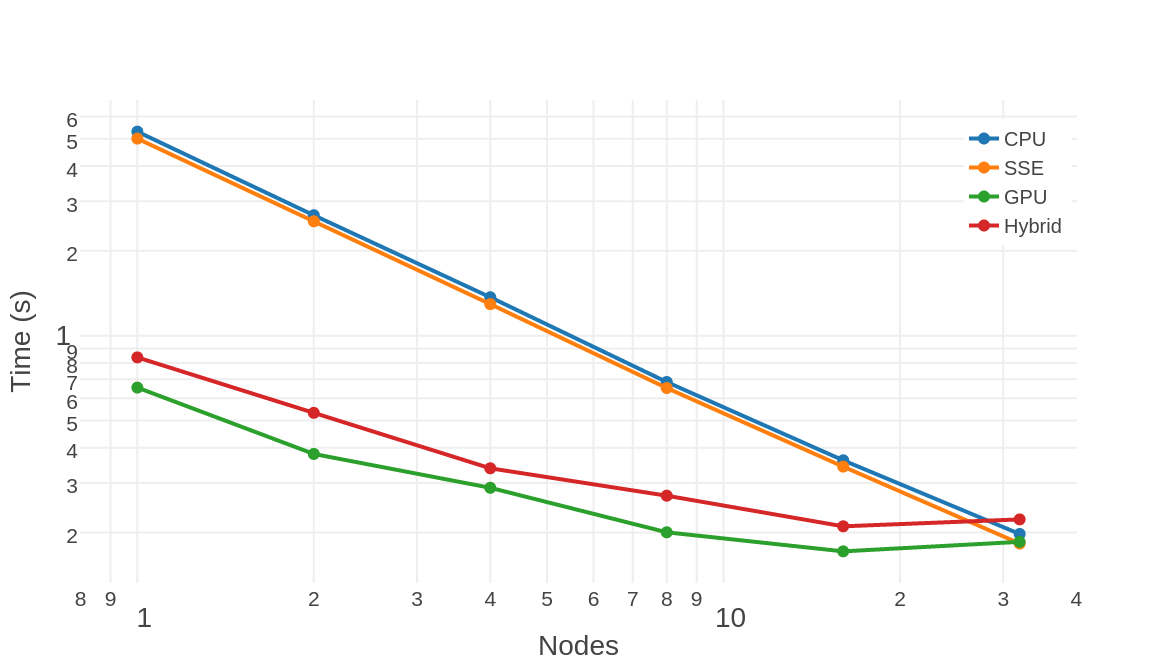
\includegraphics[width=11cm]{Plots/4096.png}
   \caption{Execution time for linear system size: 4096.} \label{plot:bench-4096}

   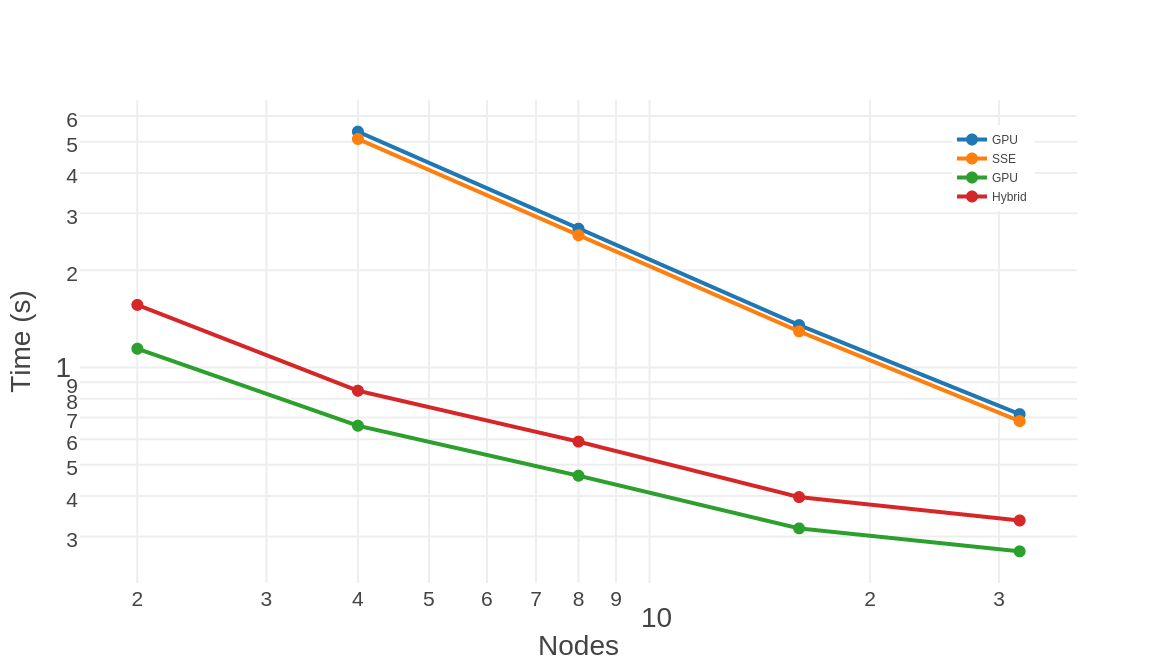
\includegraphics[width=11cm]{Plots/8192.png}
   \caption{Execution time for linear system size: 8192.} \label{plot:bench-8192}

   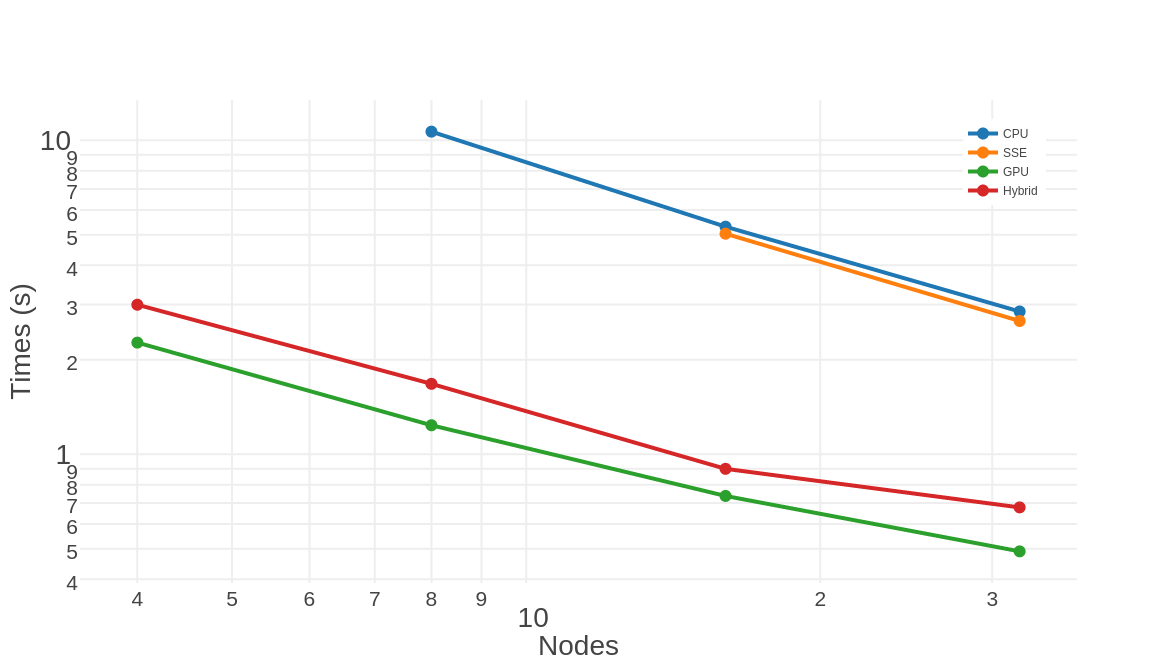
\includegraphics[width=11cm]{Plots/16384.png}
   \caption{Execution time for linear system size: 16384.} \label{plot:bench-16384}
\end{figure}
